\chapter{Spatial Metadata Discovery \& Publishing}

Once the geo-servers are crawled from the open web, we need to organize this data into a well organized manner so that it can be retrieved efficiently. The operation and query we perform on this data must be performed in a efficient manner. The aim of Spatial metadata catalog server is to make crawled spatial metadata available for public.

\section{Objectives}

\begin{enumerate}
    \item Parse the crawled metadata and store it into a permanent database in a structured manner.
    \item Publish metadata repository in OGC compliant manner to make it available as a service.
\end{enumerate}

\section{Architecture of Catalog Service}

 There are various data repositories available on the web. However this repositories are not indexed. Spatial web crawler crawls through open web and stores corresponding metadata information about available data into the xml files. Crawler uses \textit{GetCapabilities()} OGC request to find if a given server is geoserver or not, if the given URL is indeed a geo-server then crawler module requests to retrieve \textit{capabilities.xml} file from the server and stores it into warehouse. XML files contains the services information provided by the geo-servers found on the web. They are usually called services.xml.
 \begin{figure}[H]
 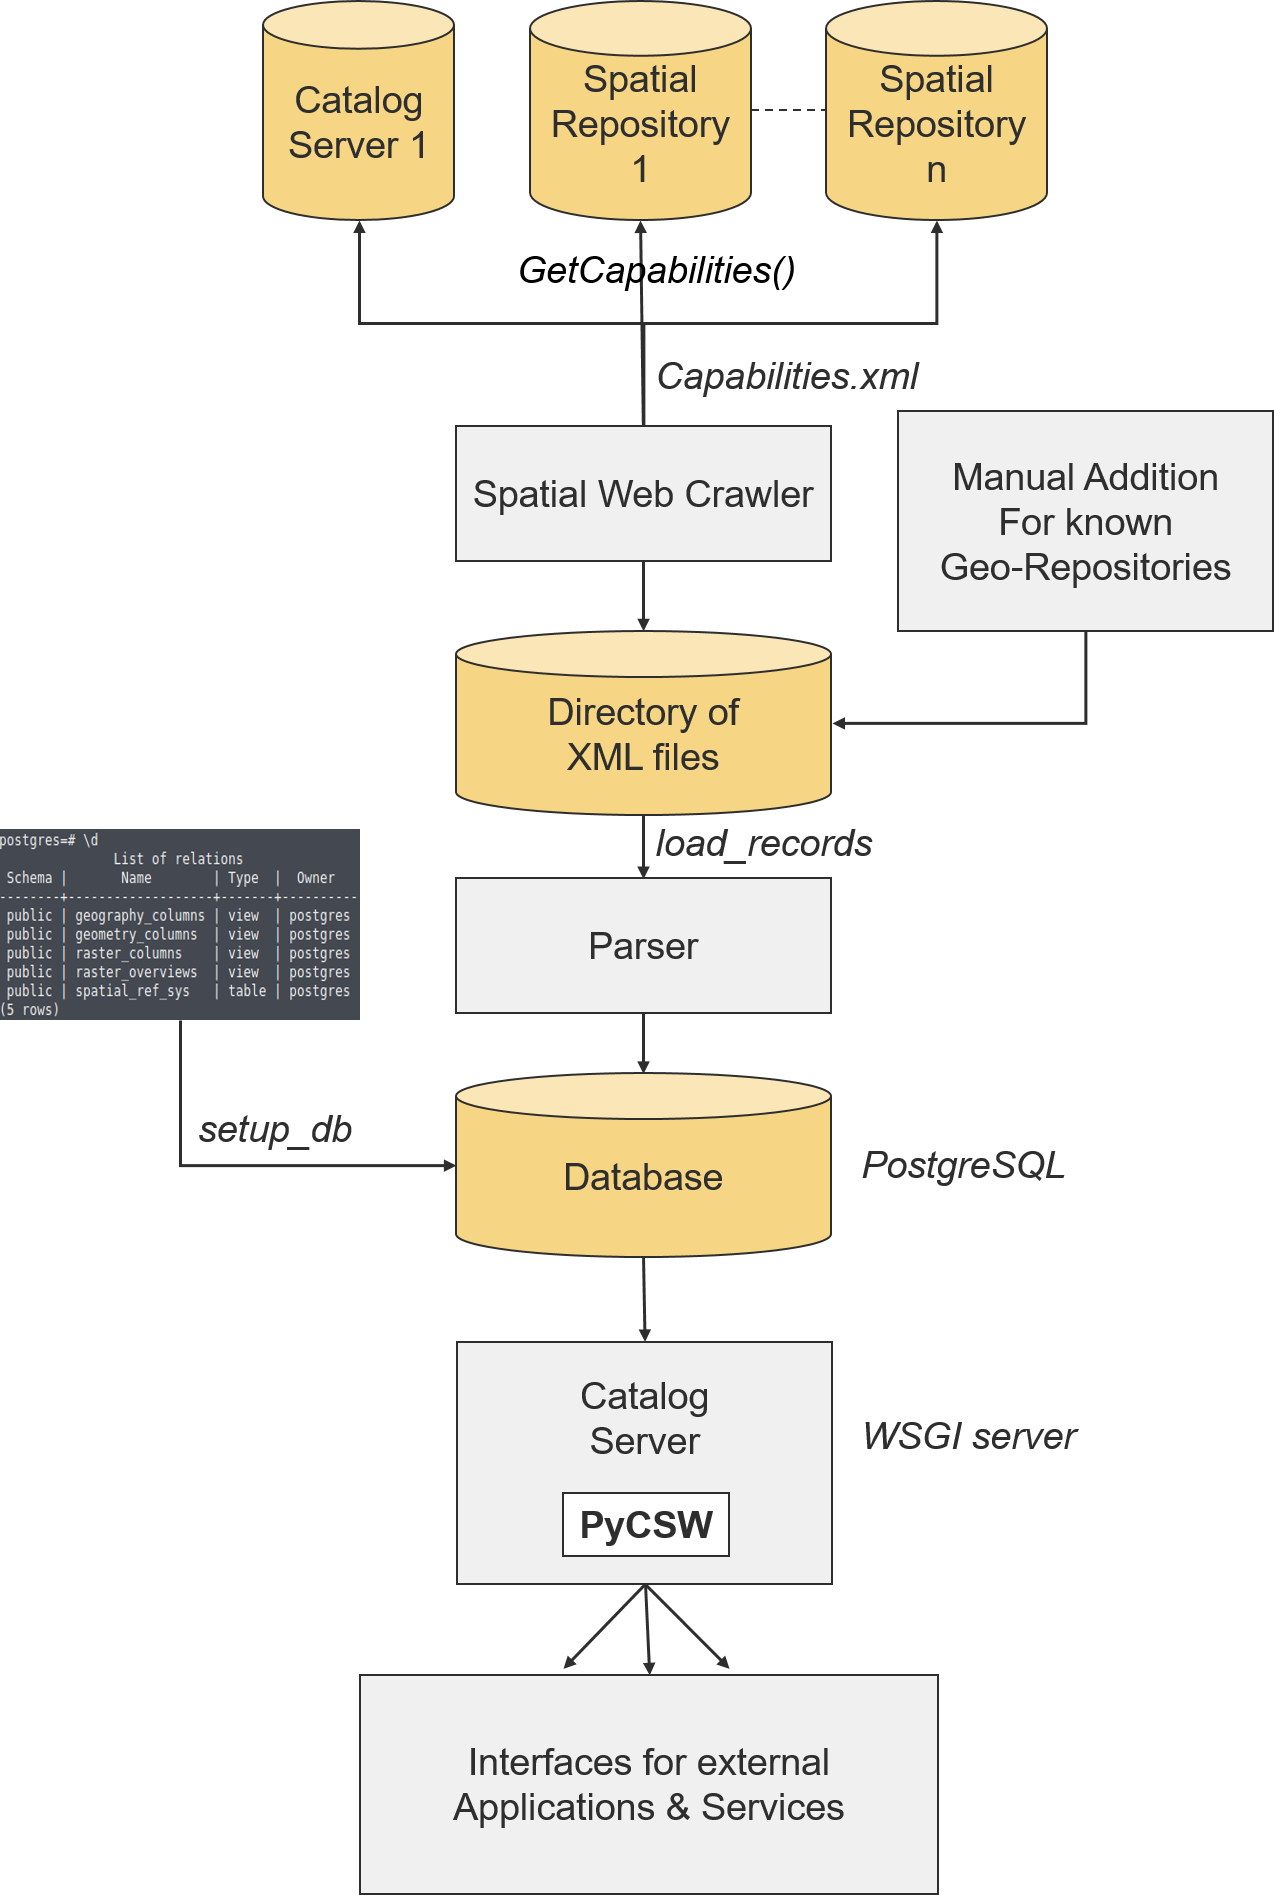
\includegraphics[width=\textwidth]{pix/Picture3}
 \caption{Architecture of Catalog Server}
 \end{figure}
 This information contains available operations, available layers and other useful information. This xml files are gathered in a folder containing xml files.\\



% \begin{figure}[h]
%   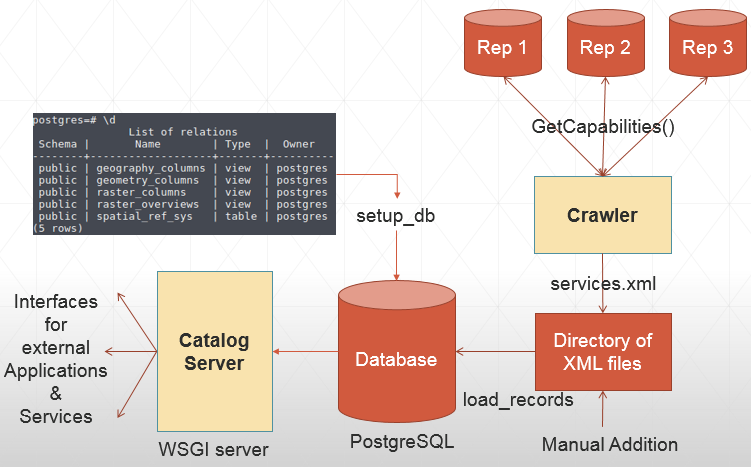
\includegraphics[width=\textwidth]{7}
%   \caption{Architecture of Catalog Service}
% \end{figure}

\par No of spatial repositories in the web is significantly lower than other type of services and servers. It can happen that it might take a significant amount of time to gather practically good number of geo-servers. For this reason, this files can be added by the spatial web crawler or it can be added manually.
\newline
\par This xml files are then loaded into the database for faster and efficient retrieval operation. For database we can use either of MySQL, PostgreSQL or SQLite. But MySQL and SQLite does not offer inherent data structures and operations support for spatial data. SQLite is also meant for light weight databases, whereas here the no of request-reply and data transfer can be very high. For these reasons it is better to choose PostgreSQL database system to store data for the catalog service. PostgreSQL offers high scalability and offers inherent support of spatial data types and operations.\newline
\par Catalog Service is hosted on \textit{Web server gateway interface (WSGI)} server. We can also use other deployment servers like Apache. Main reason for choice of server as WSGI is that, WSGI integrates well with python. It is build on python. It is useful for request-reply type ordinary web interfaces and it is efficient for file transferring on other protocols. A python program admin.py is hosted on WSGI server, which takes the metadata information from the database and replies in response to GetCapabilities() request. When working on a particular request for a repository like GetMap(), the catalog service acts as a mediator between client and the repository on which the data is hosted. It converts the request taken by WSGI server converts it into standard OGC compliant WMS or WFS call, and accesses data from original repository from where data is hosted.


\section{Implementation}
There are two types of implementation done to implement catalog service module. First implementation covers $PyCSW$ python catalog service for web and second implementation makes use of $GeoServer$ open source tool for sharing spatial data. Difference between two type of tools is while PyCSW offer great functionalities and most of the OGC compliant services, GeoServer also offers more data type support to load repository from and a management console for admin to maintain Geo-registry. We will take a look at both type of solutions here.

\subsection{Crawler Module}

In first stage implementation, we first crawl through open web using the spatial web crawler discussed in the above chapter. The crawler checks if the given server provides geospatial services or not. If the server is a geospatial repository then it collects all the metadata information about the repository and stores it in a form of a xml files. Standard OGC compliant service calls are used for collecting metadata information about found registry. Here in the figure we can see there are three repositories which have been crawled by the crawler. The information about these repositories are stored in a xml files called services.xml. The no of geoservers and registries are very less in the open web compared to other kind of services, for this reason it might take a long time to crawl and find significant amount of registry services for our catalog service. To handle this problem, manual addition option is used. We can manually add popular geoservers and registry services to the services.xml files. We know that geoservers reply in xml response when called for a $GetCapabilities$ request. We can use this property and manually add popular geo-registries beforehand to the set of xml files. So in the summary, the first stage crawls the web and stores corresponding set of services files into one place.
\newline
\par For this, python based crawler module program is used. It takes a set of seed URLs, checks if the URL can built object of OGC compliant WMS or WFS object. If it can build OGC WMS object then, crawler requests for capabilities file, and stores it in set of xml files.


\subsection{Database Setup}
In second step, These set of xml files are used to populate database. Here various type of databases can be used. I have tried databases like MySQL, SQLite and PostgreSQL. In our approach I have used PostgreSQL because it offers geospatial properties and services inherently. Other databases do not offer inbuilt services for spatial data. PostgreSQL database offers PostGIS extension, which are a set of libraries to extend PostgreSQL database into spatial database. For adding PostGIS to PostgreSQL, go to PostgreSQL shell psql and create a extension, PostGIS. 

\begin{center}
\textit{CREATE EXTENSION POSTGIS;}
\end{center}

\par Once this is done, import all of the services,xml files into the database. Create structured tables and schema for maintaining spatial data. For this purpose \textit{setup\_db} command is used from catalog service module.

\begin{figure}[h]
\centering
  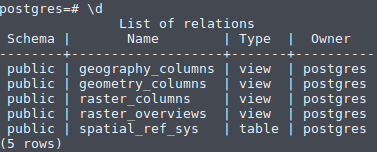
\includegraphics[width=0.8\textwidth]{8}
  \caption{List of relations}
\end{figure}

\par Here four tables are built to store and index spatial data efficiently. Those are, $geometry\_columns, records$ , $spatial\_ref\_sys$ and $spatial\_ref\_sys\_srid\_seq$. This tables are then used by the catalog server to publish and query available data. When a external entity queries catalog server for Get Capabilities request, the catalog server replies with the services file which contains all the information about all the geo-servers it has crawled till now. Thus it contains all the layer information and data crawled from the Internet. This makes it a single point of resource access. Data from xml files is parsed and stored into respective relations. For this \textit{load\_records} command is used from admin.py module within PyCSW. These tables are used to store parsed spatial features from the spatial repositories.

\subsection{Catalog Service}
Catalog service takes all available data from the database and creates a metadata capabilities file. It acts as a mediator between repositories which actually contains the data and the client. When a client requests for a query or a metadata service, catalog service checks if the database contains the information. If metadata information is requested, it replied directly to the client with the necessary files or response.\\
\begin{figure}[h]
\centering
  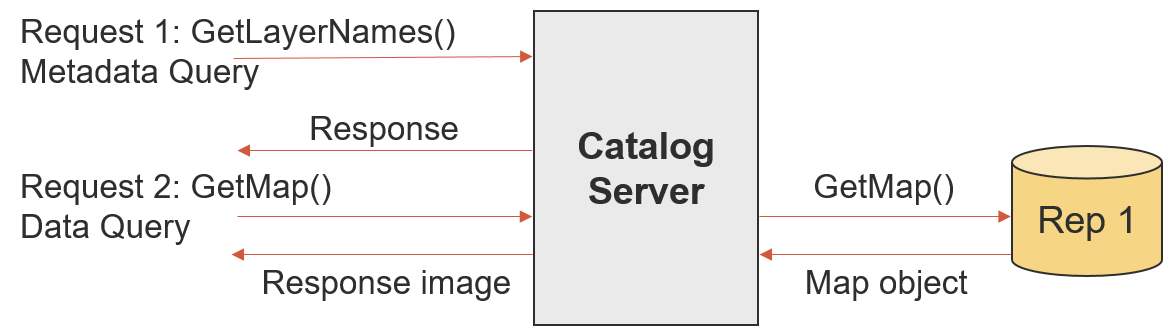
\includegraphics[width=\textwidth]{pix/Picture5}
  \caption{Catalog Service as a mediator}
\end{figure}
\par In case of query requiring actual data instead of the metadata, the catalog service resolves the source from which the data is available and brings the data back to the requester client. In this case, the catalog service acts as a mediator between client and the data source, acting just as a catalog. Here the catalog service is implemented via GeoServer. GeoServer takes the crawled layers from web map service and loads it into catalog.

\subsection{Query Processing}
When a query or request for the data is processed by the catalog service, it acts as a mediator between client and the repository from which the data is intended. It creates a object of the required service and requests for the object on behalf of the client. Client authorizes to the catalog service and catalog service authorizes itself to the data repositories for the transfer of data. Catalog service takes the object response from the repository and send it in response to client in client specified format. For metadata queries the catalog service retrieves data from database via object relational mappings in programming paradigms, this helps when having a multiple references to same object or feature. This method is used for retrieval of the features. How the featured are retrieved and presented are discussed further in the chapter 5.


%%%%%%%%%%%%%%%%%%%%%%%%%
\section{Extending catalog service with cloud characteristics}
A key logical step to scale catalog service for the larger audience is to make a cloud based implementation. Cloud based implementation has characteristics like scaling horizontally, high availability and dynamic dispatch of machines. To achieve the effects of scalability and high availability, we can make use of $load\_balancer$, $load\_balancer$ is a machine that acts as a middleware between client request and actual catalog servers. It forwards the request to one of the servers based on some qualitative features.
\newline
\begin{figure}[h]
    \centering
    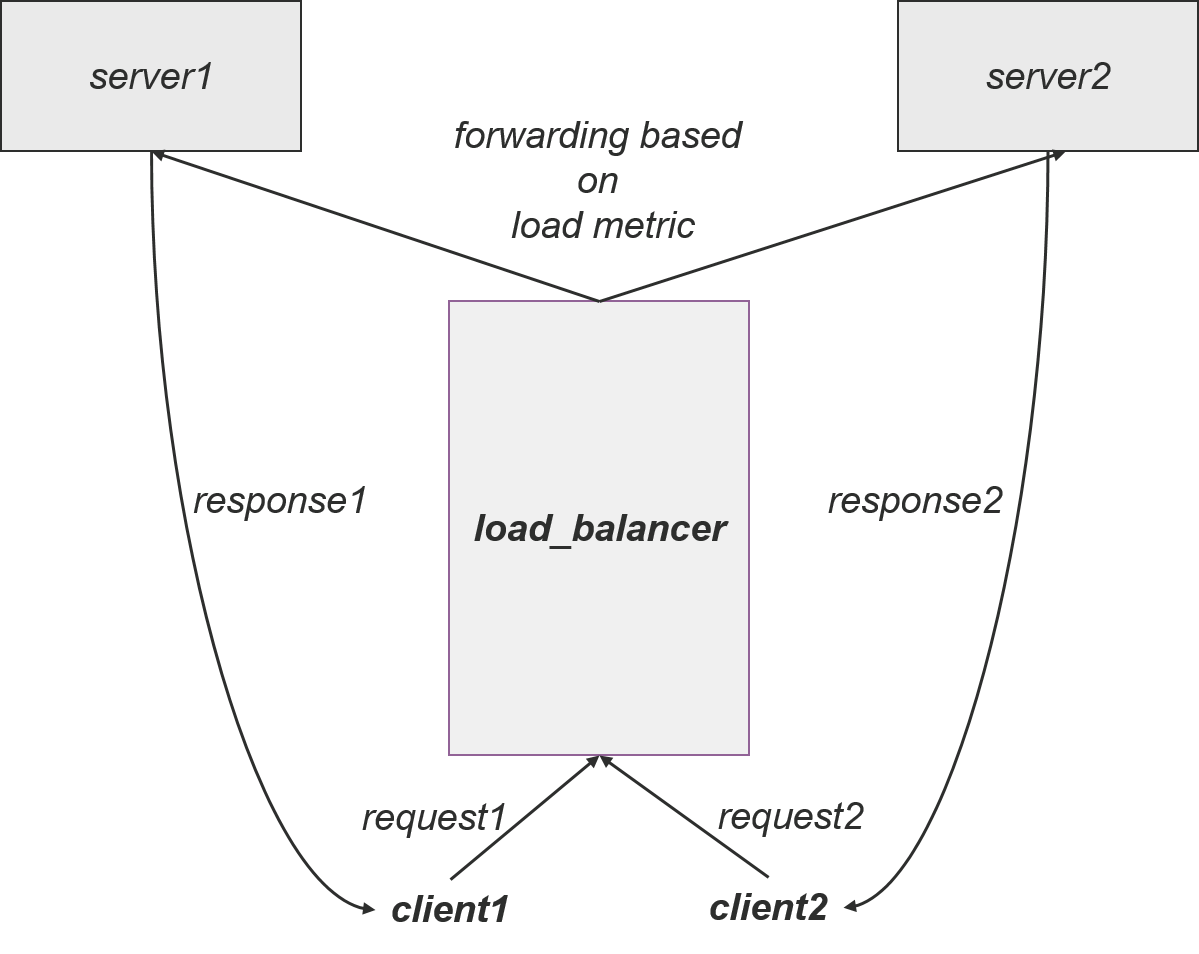
\includegraphics[width=0.7\textwidth]{pix/Picture7}
    \caption{load balancer implementation}
    \label{p7}
\end{figure}


\par In our approach, we have started by building a $load\_balancer$ which balances the requests between multiple available given geoservers. These geoservers are cloned to provide similar functionality but high availability. $load\_balancer$ detects which server has low number of requests compared to others and forwards the request to particular server. Actual servers are transparent to the end users. Interface between client and the geoservers is the $load\_balancer$. It acts as a gateway for connecting with the geoservers. In our test implementation, we have created two instances of geoservers and run similar repositories on each of them. The client connects to the $load\_balancer$ which acts as a gateway for the actual geoservers. It gets the reply back from the actual servers and sends it to requesting clients. $load\_balancer$ can also restrict or allow certain users grant on certain function and not all of them, thus here $load\_balancer$ also acts as a control panel and authorization entity for the access control.
\newline
\begin{figure}[h]
    \centering
    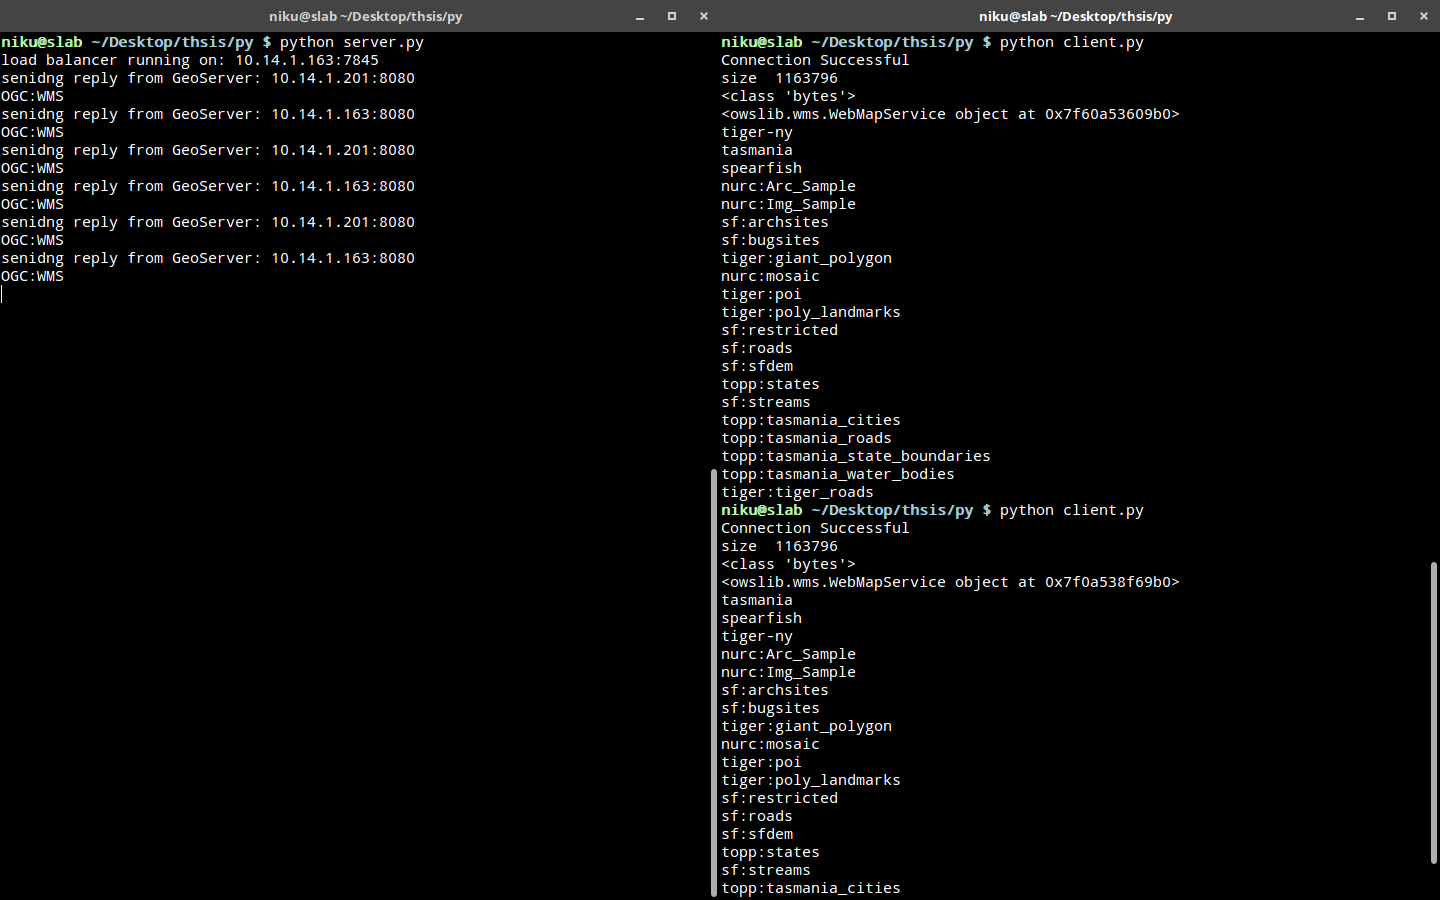
\includegraphics[width=\textwidth]{pix/p13}
    \caption{load balancer preliminary results}
    \label{p13}
\end{figure}
%%%%%%%%%%%%%%%%%%%%%%%%%
\section{Results}
Here are some results from the projects that explains and elaborates what kind of information can be get from catalog service. We have connected to GeoServer instance that is locally hosted. Note that many more richer services can be added to the platform to extend it's functionality.

\begin{figure}[h]
    \centering
    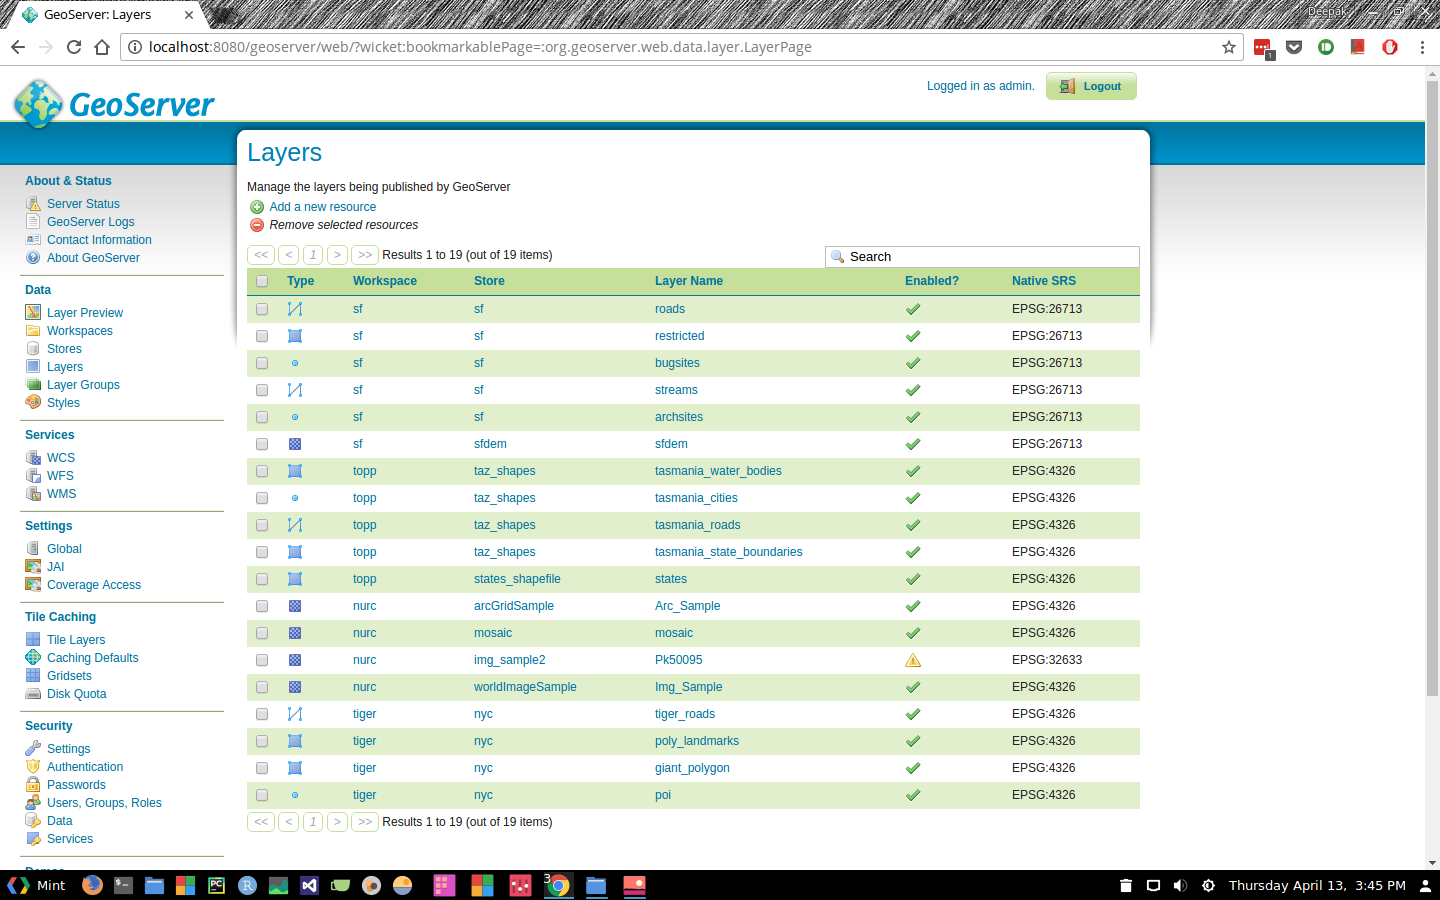
\includegraphics[width=\textwidth]{pix/p8}
    \caption{GeoServer Implementation}
\end{figure}

\begin{itemize}

\item Information about service metadata : OGC:WMS\\
This shows that registry is capable of providing OGC compliant web map service type of service to the user.\\

\item Title : GeoServer Web Map Service\\
Title gives information about title of the server hosting web map service.

\item List of available layers
\begin{enumerate}
\item kgp:POPULATION 
\item kgp:bnk\_block\_boundary 
\item kgp:bnk\_block\_hq 
\item kgp:bnk\_district\_boundary 
\item kgp:bnk\_drainage 
\item kgp:bnk\_grampanchayat\_boundary 
\item kgp:bnk\_mouza\_boundary 
\item kgp:bnk\_road
\item tasmania
\item spearfish
\item tiger\-ny
\item nurc:Arc\_Sample
\item nurc:Img\_Sample
\item sf:archsites
\item sf:bugsites
\item tiger:giant\_polygon
\item nurc:mosaic
\item tiger:poi
\item tiger:poly\_landmarks
\item sf:restricted
\item sf:roads
\item sf:sfdem
\item topp:states
\item sf:streams
\item topp:tasmania\_cities
\item topp:tasmania\_roads
\item topp:tasmania\_state\_boundaries
\item topp:tasmania\_water\_bodies
\item tiger:tiger\_roads
\end{enumerate}

This shows the list of available data in the form of layers. Each layer represents data of a geographic location from a view point. Multiple layers can be overlapped on each other to better understand the data. Each layer contains multiple features in itself. 

\item Available operations (WMS)
\begin{enumerate}
\item GetCapabilities 
\item GetMap 
\item GetFeatureInfo 
\item DescribeLayer 
\item GetLegendGraphic 
\item GetStyles 
\end{enumerate}

Gives details about the operations that can be performed by the geoserver. For example, DescribeLayer provides information about a particular layer. GetMap returns a map of layer in multiple available formats. 

\item GetMap\\
\begin{figure}[H]
	\centering
  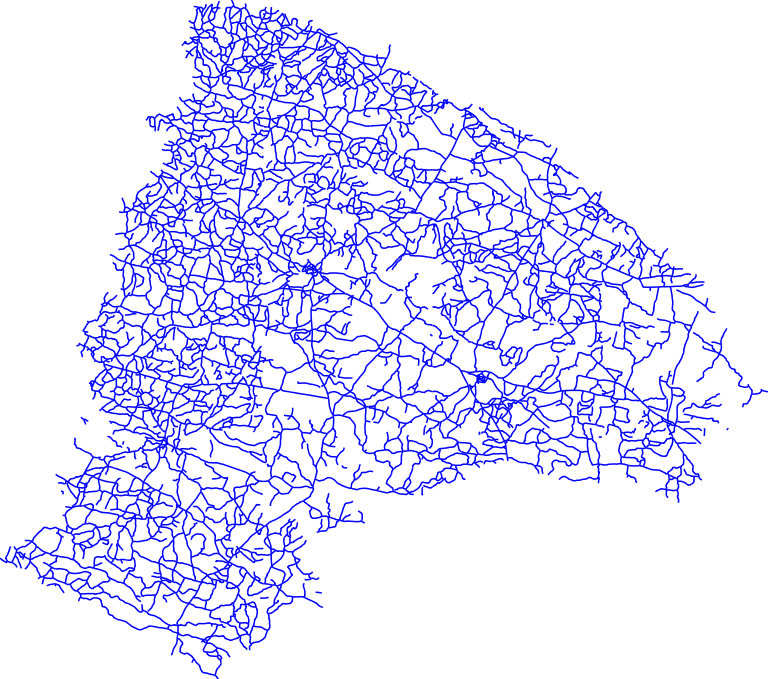
\includegraphics[width=0.7\textwidth]{bnk}
	\caption{Map of KGP BNK ROAD}
\end{figure}
Returns a map of particular layer. Can be superimposed to another map for better visualization. GetMap supports multiple options like name of layer(s), styles, transparency, bounding box, size and format like jpeg, png or pdf. 
\item DrawMap\\
DrawMap overlays different map images on top of each other to better visualize and analyze the effect of desired operation. For example, it can be used to find area affected by flood, or to find division of regions based on religion.\\
\begin{figure}[H]
	\centering
  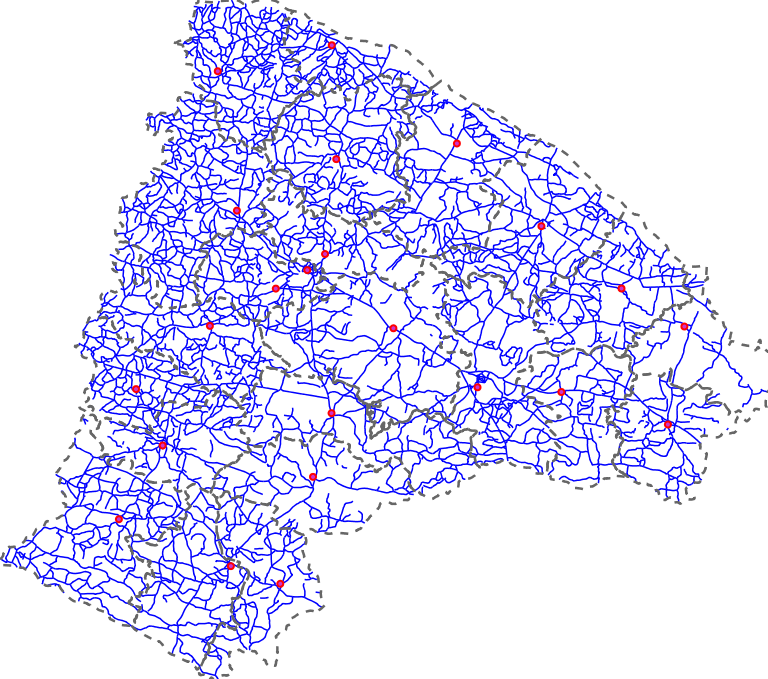
\includegraphics[width=0.7\textwidth]{9}
	\caption{Overlay of KGP BNK ROAD, Block HQ \& Boundary Layers}
\end{figure}
User can specify options to get the result image in desired format.\\
Options:\\
Layers = \{ kgp:bnk\_road, kgp:bnk\_block\_hq, kgp:bnk\_block\_boundary \}\\
Width = 768\\
Height = 679\\
Format = image/png

\item Information about specific layer: 
\begin{itemize}
\item Title --- POPULATION 
\item Name --- kgp:POPULATION 
\item Is Queryable --- 1 
\item Is Opaque --- 0 
\item Bounding Box ---  
\item minx --- 68.52669525146484 
\item miny --- 8.086045265197754 
\item maxx --- 97.3387680053711 
\item maxy --- 35.8697509765625
\end{itemize}
Provides information about a particular layer, for example, name of the layer, title, bounding box information etc.

\item Similar information can be found for web feature service, for example, supported operations in WFS.
\begin{enumerate}
\item GetCapabilities
\item DescribeFeatureType
\item GetFeature
\item GetGmlObject
\item LockFeature
\item GetFeatureWithLock
\item Transaction
\end{enumerate}

\end{itemize}
